\subsection{Virtual heart and pacemaker models}
\label{heartmodel}

Since we don't have access to real human hearts for testing, we have developed a \emph{Virtual Heart Model (VHM)}, which simulates the \emph{timing aspects} of the operation of a human heart, and ignores other physiological details.
\todo[inline]{ZJ : review following for accuracy}
The VHM uses Finite State Machine (FSM) to model seven locations in the heart, in particular the following: the SA node, the AV node, and the ventricle.
The paths connecting them are also modeled as FSMs.
These FSMs capture the operating modes of the nodes (depolarizing, refractory, idle) and those of the paths (conducting, backward-conducting, etc.), as well as the conditions leading from one state to another (e.g. a path conduction is followed by the node entering the depolarized state).
See Fig.~\ref{fig:FSMSA} for an example of a node FSM.
\begin{figure}[t]
\centering
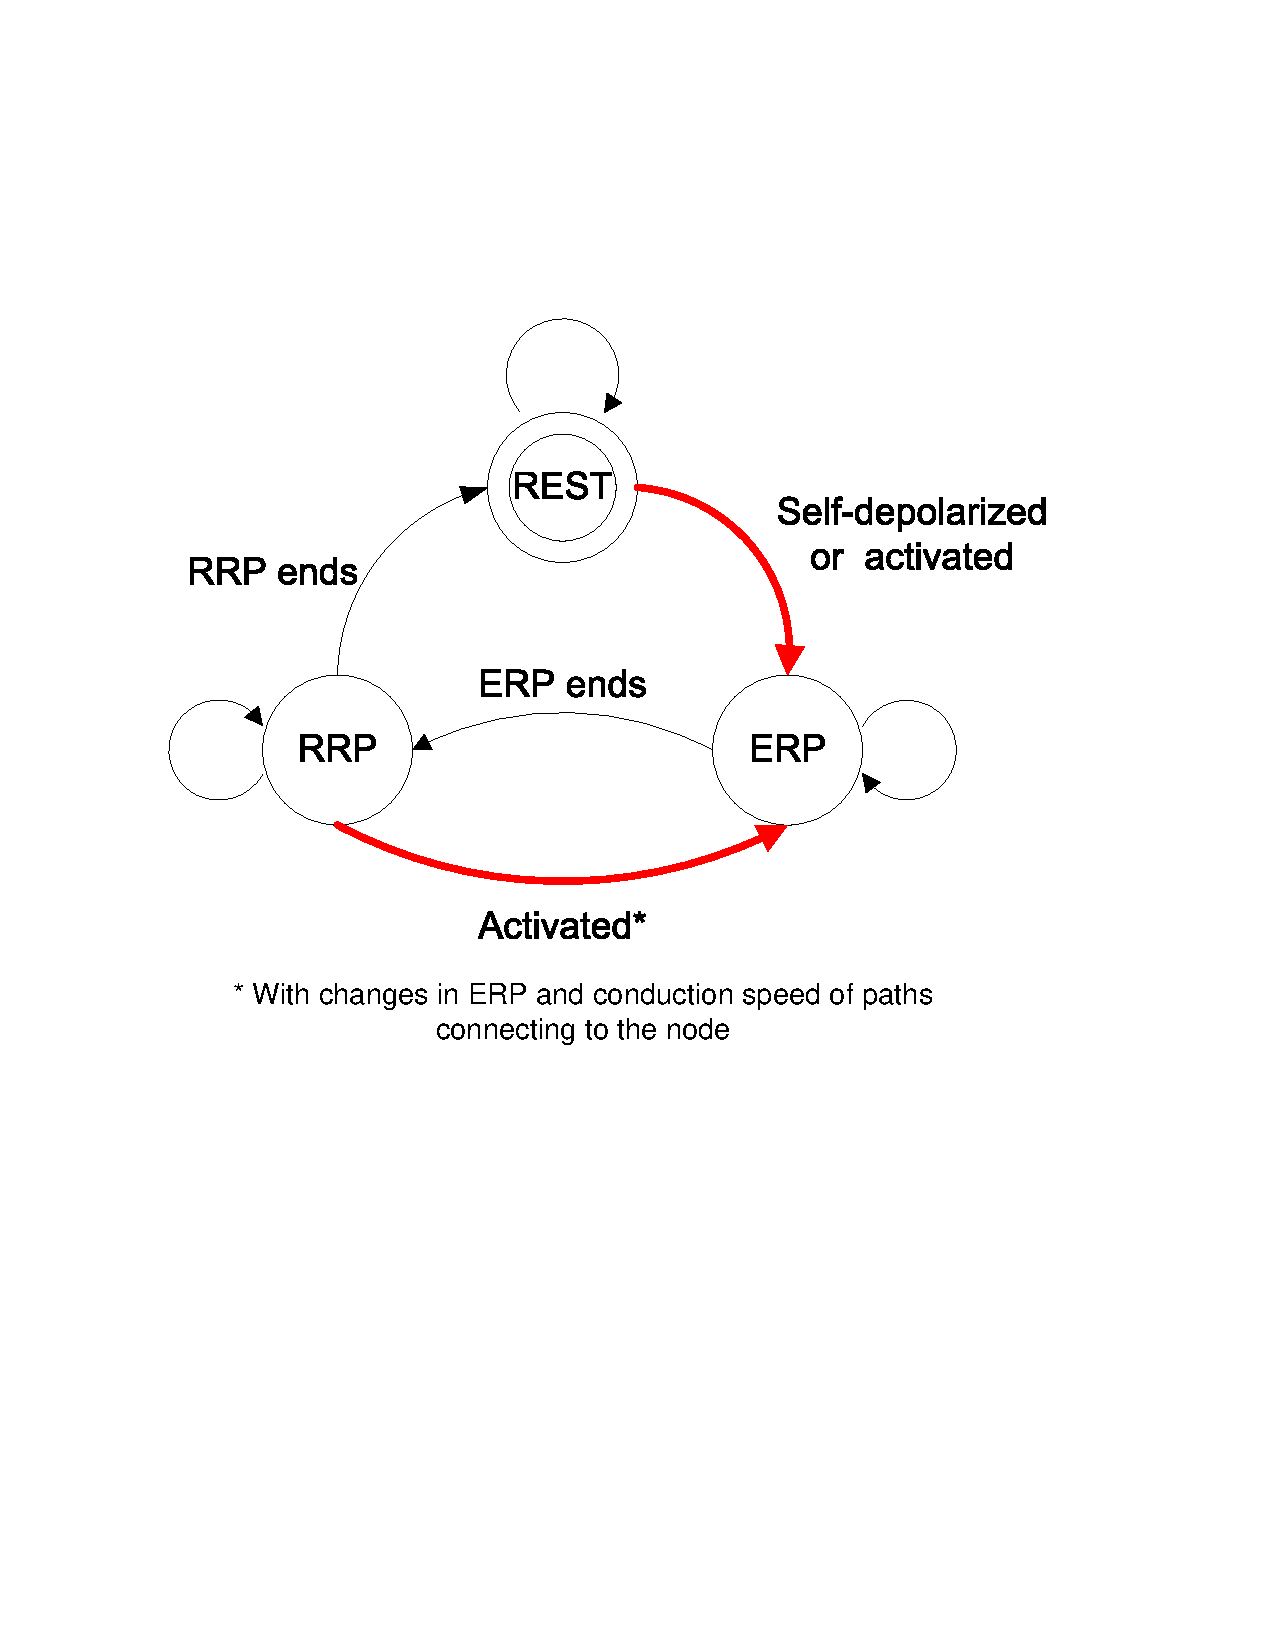
\includegraphics[scale=0.4]{node_automata.pdf}
\caption{FSM modeling the SA node showing Effective and Relative Refractory Periods (ERP and RRP) and the Rest state.}
\label{fig:FSMSA}
\end{figure}
The VHM is implemented in both Simulink and Matlab. 
We used the VHM to simulate different heart conditions in a closed loop with the pacemaker model, such as Wenckebach AV nodal response, atrial flutter and pacemaker mediated tachycardia.
The VHM functional output has been validated by the director of cardiac electrophysiology in the Philadelphia VA Hospital and by electrophysiologists in the Hospital of the University of Pennsylvania. 
More details are available in \cite{VHM_proc}.

To run the experiments in this paper, we used a DDD pacemaker model developed according to the specification derived from the Boston Scientific Challenge~\cite{challenge}.
%\todo[inline]{ZJ : 2-3 lines describing the PM model.}
The model has been verified against the specifications using open-loop testing \cite{testing}. Local electrical impulses in the atrium and the ventricle can trigger $AS$ and $VS$ events, respectively. The pacemaker can deliver electrical pacing from the atrial lead ($AP$) and the ventricular lead ($VP$). The most basic functions of a DDD pacemaker is described as follow: From any ventricular events (VS,VP), if no AS appear within $TLRI-TAVI$, the pacemaker will deliver AP. From any atrial events (AS,AP), if no VS appear within $TAVI$ and the interval from the last ventricular event (VS,VP) is longer than $TURI$, the  pacemaker will deliver VP. Together these two functions guarantee the ventricular rate of the heart maintained above $60000/TLRI$ bpm and the paced ventricular rate is lower than $60000/TURI$ bpm.
%More information about the implementation can be found in \cite{testing}. 

%\textbf{1. Lower Rate Interval (LRI)}:
%The LRI interval starts at a ventricular sensed or paced event. The LRI interval is the longest interval between two ventricular events. 
%
%\textbf{2. Upper Rate Interval (URI)}:
%The URI interval defines the shortest interval between a ventricular event and a paced ventricular event
%
%\textbf{3. Atrial-Ventricular Interval (AVI)}:
%Ventricular pacing shall occur in the absence of a sensed ventricular event within the programmed AV delay when the time elapsed after the last ventricular event is between the programmed LRI and URI.
%
%\textbf{4. Ventricular Refractory Period (VRP)}:
%The VRP is the time interval following a ventricular event during which no ventricular sense (VS) can happen.
%
%\textbf{5. Post Ventricular Atrial Refractory Period (PVARP)}:
%The PVARP is the time interval following a ventricular event during which no atrial sense (AS) can happen.
%
%According to the five primary specifications of the basic DDD pacemaker, a Simulink model was designed using temporal logic. Each component corresponds to a particular specification and communicates with others using channels. A timing diagram is shown in \ref{timingPM}. 
%%%%%%%%%%%%%%%%%%%%%%%%%%%%%%%%%%%%%%%%%%%%%%%
%\begin{figure}[!b]
%	\center
%	\vspace{-10pt}
%	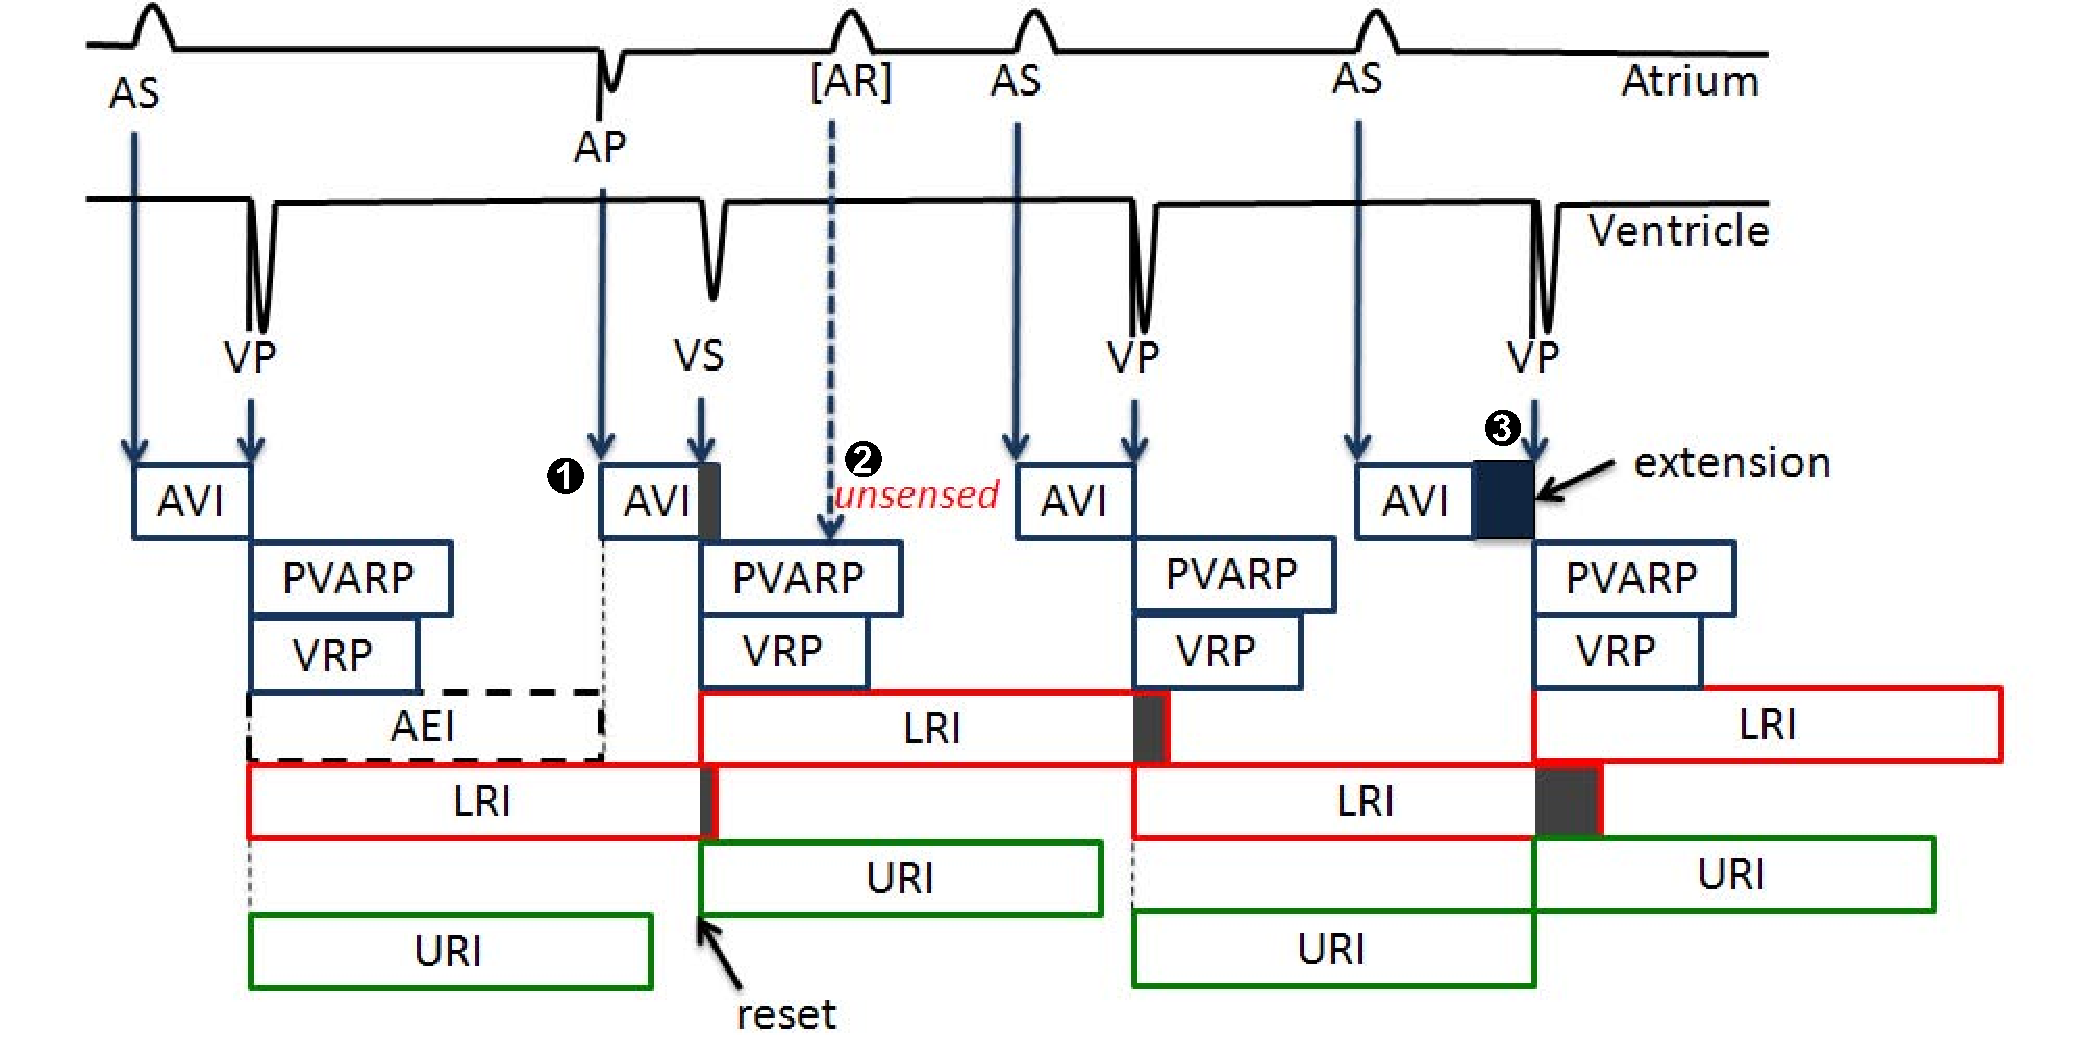
\includegraphics[width=0.45\textwidth]{figures/PM_timers.pdf}
%	\vspace{-10pt}
%	\caption{Simulink design of path automata}
%	\label{fig:timingPM}
%\end{figure}